\documentclass[12pt]{article}

%% Language and font encodings
\usepackage[english]{babel}
\usepackage[utf8x]{inputenc}
\usepackage[T1]{fontenc}
\usepackage{float}

%% Sets page size and margins
\usepackage[a4paper,top=3cm,bottom=2cm,left=3cm,right=3cm,marginparwidth=1.75cm]{geometry}

%% Useful packages
\usepackage{amsmath}
\usepackage{graphicx}
\usepackage[colorinlistoftodos]{todonotes}
\usepackage[colorlinks=true, allcolors=blue]{hyperref}

% \title{Assembler-Linker-Loader Simulation}
%%\author{You}

\begin{document}
\begin{titlepage}
    \begin{center}
        \vspace*{8cm}
        
        \Huge
        \textbf{Simulation of Assembler-Linker-Loader}
        
        \vspace{1.0cm}
        \LARGE

        
        \vspace{0.2cm}
        
        \textbf{CS-244}
        
%         \vfill
        
        
    \end{center}
\end{titlepage}
 \newpage
\tableofcontents
\newpage

\section{Introduction}

This assignment is a part of CS-244(System programming laboratory) course, in which we had to make a simulator for parser,assembler,linker,and loader for a programming language.\\
A  computer  will  not  understand  any  program  written  in  a 
language,  other  than  its  machine  language.  The  programs  written  in  other 
languages  must  be  translated  into  the  machine  language.  Such  translation 
is  performed  with  the  help  of  software.  A  program  which  translates  an 
assembly  language  program  into  a  machine  language  program  is  called  an 
assembler.\\In  high  level  languages,  some  built  in  header  files  or  libraries  are 
stored.  These  libraries  are  predefined 
and  these  contain  basic  functions 
which are essential for executing the program. These functions are linked to 
the libraries by a program called Linker. Usually  a  longer  program  is  divided  into  smaller 
subprograms  called  modules.  And  these  modules  must  be  combined  to 
execute the program. The process of combining the modules is done by the 
linker.\\Loader is a program that loads machine codes of a program into the 
system   memory.In Computing,   a loaderis   the   part   of   an Operating  System
that  is  responsible  for  loading  programs.  It  is  one  of  the  essential 
stages in the process of starting a program. Because it places programs into 
memory  and  prepares  them  for  execution.Below is the figure showing the hierarchy of execution of a computer program beginning of a c code.

\begin{figure}[!htb]
\centering
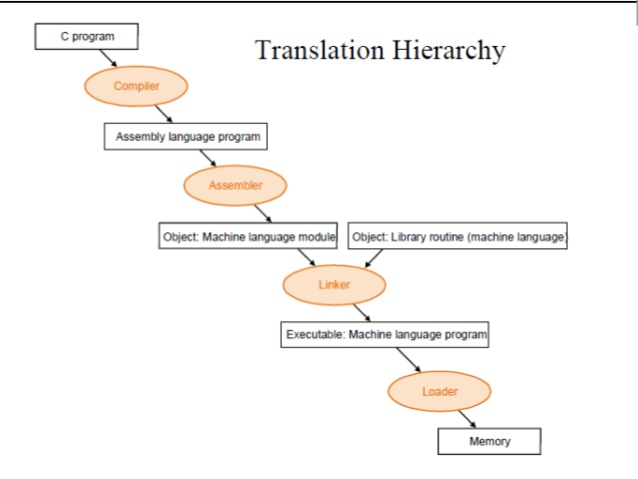
\includegraphics[width=0.7\textwidth]{hierarchy_assemble.jpg}
\caption{\label{fig:hierarchy}Hierarchy of execution of a program.}
\end{figure}

\section{Components related to this Assignment}

\subsection{Scanning and Parsing}
Scanning is the process of recognizing the lexical components in a source strings.
A Scanner simply turns an input String (say a file) into a list of tokens. These tokens represent things like identifiers, parentheses, operators etc.\\
The goals of parsing are to check the validity of a source string,and to determine its syntactic structure.For the invalid string, the parser issues diagnostic messages reporting the cause and nature of error(s) in the string.For a valid string(code statement in this case),it builds a parse tree to reflect the sequence of derivations or reductions performed during the parsing.
A parser converts this list of tokens into a Tree-like object to represent how the tokens fit together to form a cohesive whole (sometimes referred to as a sentence).


In terms of programming language parsers, the output is usually referred to as an Abstract Syntax Tree (AST). Each node in the AST represents a different construct of the language, e.g. an IF statement would be a node with 2 or 3 sub nodes, a CONDITION node, a THEN node and potentially an ELSE node.\\
\textbf{Parse trees and Abstract syntax trees}\\
A parse tree depicts the steps in parsing, so it is useful for understanding the process of parsing.However it is a poor intermediate representation of a source string because it contains too much information as far as subsequent processing in the compiler is concerned.An abstract syntax tree(AST)  represents the structure of a source string in a more economical manner.The word 'abstract'  implies that it is a representation designed by a compiler designer for his own purposes.
Below is the diagram representing the process of parsing and scanning of programming code lines.



\begin{figure}[!htb]
\centering
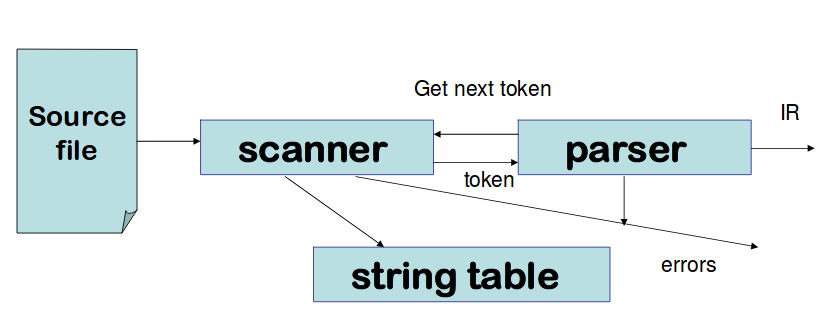
\includegraphics[width=0.7\textwidth]{scanning-and-parsing.png}
\caption{\label{fig:sc_pa}Scanning and parsing of code lines.}
\end{figure}
In our case,we have scanned the code lines using regex library in python for all types of statements available in the language which we designed according to the syntax so defined for each.For a given programming statement, it firts tokenizes and checks against all defined regexes.Defition of some regexes can be seen in the table below.
\begin{table}[!htb]
\centering
\begin{tabular}{l|r}
Operation & Regex Definition \\\hline
Addition &  \verb|\s*(\w+)\s*=\s*(\w+)\s*\+\s*(\w+)\s*|  \\
Extern Variable &    \verb|extern\s+(\w+)\s*|   \\
Loop &    \verb|\s*loop\s+(\w+)\s*|   \\
Macro  &    \verb|\s*macro\s*|   \\
Minimum of a list\\    e.g., min(2,3,0,1) & \verb|\s*(\w+)\s*=\s*min\s*\((.*)\)\s*|
\end{tabular}
\caption{\label{tab:regex}Some regex definitions in python.}
\end{table}


One of the most important uses of the theory of formal languages is in the definition of programming
languages and in the construction of interpreters and compilers for them. The basic problem here is to
define a programming language precisely and to use this definition as the starting point for the writing
of efficient and reliable translation programs. Both regular and context-free languages are important
in achieving this. As we have seen, regular languages are used in the recognition of certain simple
patterns that occur in programming languages, but as we argue in the introduction to this chapter, we
need context-free languages to model more complicated aspects.\\As with most other languages, we can define a programming language by a grammar. It is
traditional in writing on programming languages to use a convention for specifying grammars called
the Backus-Naur form or BNF. This form is in essence the same as the notation we have used here,
but the appearance is different. In BNF, variables are enclosed in triangular brackets. Terminal
symbols are written without any special marking. BNF also uses subsidiary symbols such as |, much
in the way we have done.\\Many parts of C-like programming languages are susceptible to definition by restricted forms of
context-free grammars. For example, the while statement in C can be defined as
Here the keyword while is a terminal symbol. All other terms are variables, which still have to be
defined.\\Unfortunately, not all features of a typical programming language can be expressed by an s-
grammar. The rules for
above are not of this type, so that parsing becomes less
obvious. The question then arises what grammatical rules we can permit and still parse efficiently. In
compilers, extensive use has been made of what are called LL and LR grammars. These grammars
have the ability to express the less obvious features of a programming language, yet allow us to parse
in linear time.\\In connection with this, the issue of ambiguity takes on added significance. The specification of aprogramming language must be unambiguous, otherwise a program may yield very different results
when processed by different compilers or run on different systems. As Example 5.11 shows, a naive
approach can easily introduce ambiguity in the grammar. To avoid such mistakes we must be able to
recognize and remove ambiguities. A related question is whether a language is or is not inherently
ambiguous. What we need for this purpose are algorithms for detecting and removing ambiguities in
context-free grammars and for deciding whether or not a context-free language is inherently
ambiguous. Unfortunately, these are very difficult tasks, impossible in the most general sense, as we
will see later.\\Those aspects of a programming language that can be modeled by a context-free grammar are
usually referred to as its syntax. However, it is normally the case that not all programs that are
syntactically correct in this sense are in fact acceptable programs. For C, the usual BNF definition
allows constructs such as\\
char
a, b, c; followed by\\
c = 3.2;\\
This combination is not acceptable to C compilers since it violates the constraint, “a character
variable cannot be assigned a real value.” Context-free grammars cannot express the fact that type
clashes may not be permitted. Such rules are part of programming language semantics, since they have
to do with how we interpret the meaning of a particular construct.
Programming language semantics are a complicated matter. Nothing as elegant and concise as
context-free grammars exists for the specification of programming language semantics, and
consequently some semantic features may be poorly defined or ambiguous. It is an ongoing concern
both in programming languages and in formal language theory to find effective methods for defining
programming language semantics. Several methods have been proposed, but none of them has been as
universally accepted and are as successful for semantic definition as context-free languages have
been for syntax.

\subsection{Compiling to Assembly Language(.asm)}
We used the 8085 instruction set for converting the programming file to the assembly language.\\
After scanning which we did as explained in the previous section with the use of regex python expressions,each lines of code was converted to the equivalent assembly 8085 instruction.Below is the list of several operations which our program handles.\\\\
\textbf{The 8085 programming model}\\
8085 processor has a set of seven 8-bit registers including the accumulator and six others, namely, B, C, D, E, H and L. Depending upon applications, the registers other than the accumulator can be used either as independent byte-registers or as 16-bit register pairs.
A 16-bit special-purpose register called program counter is available in the microprocessor. It stores the address of the next instruction to be fetched. A 16-bit stack pointer stores the address of the last byte entered into the stack.\\
8085 is pronounced as "eighty-eighty-five" microprocessor. It is an 8-bit microprocessor designed by Intel in 1977 using NMOS technology.\\

It has the following configuration: −\\

\begin{enumerate}
\item     8-bit data bus.
\item     16-bit address bus, which can address upto 64KB.
\item     A 16-bit program counter.
\item     A 16-bit stack pointer.
\item     Six 8-bit registers arranged in pairs: BC, DE, HL.
\item     Requires +5V supply to operate at 3.2 MHZ single phase clock.
\end{enumerate}


\textbf{Addition of two numbers in our programming language:} \\
var a = 0 \\
var b = 4 \\ 
var c = a + b \\\\
Assembly file generated by our program gives:\\
MVI D, ='0'\\
MOV \#a,D\\
MVI D, ='4'\\
MOV \#b,D\\
MOV D,\#a\\
MOV \#c,D\\
END\\
a DS 1\\
b DS 1\\
c DS 1\\
='0'\\
='4'\\\\
\textbf{use of jump instruction(unconditional) :}\\
var c = 0\\
JUMP here\\
c = c + 20\\
here:\\
var c = 10\\\\
Assembly file generated by our program gives:\\
MVI D, ='0'\\
MOV \#c,D\\
JMP ~~~here\\
LDA \#c\\
ADI 20\\
STA \#c\\
MVI D, ='10'\\
MOV \#c,D\\
END\\
c DS 1\\
c DS 1\\
='0'\\
='10'\\
\\ \textbf{Similarly for the array indexing and declaration }\\
var c = 5\\
var a[5]  \\
a[1] = 1\\
a[3] = c\\\\
Assembly file generated by our program gives:\\
MVI D, ='5'\\
MOV \#c,D\\
MVI A, 1\\
STA \#a+1\\
LDA \#c\\
STA \#a+3\\
END\\
c DS 1\\
='5'\\
a DS 5\\

In this phase also(along with pass1 and pass2 phase also), different compilation/syntax errors have been found.Below are few of such instances.
% \begin{figure}[H]
% \centering
% 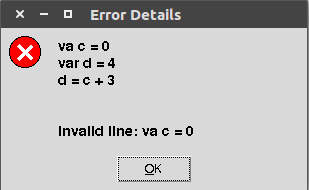
\includegraphics[width=0.5\textwidth]{error_va.png}
% \caption{\label{fig:err_va}Syntax Error}
% \end{figure}
\begin{figure}[H]
   \begin{minipage}{0.48\textwidth}
     \centering
     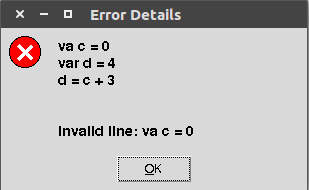
\includegraphics[width=.7\linewidth]{error_va.png}
     \caption{\label{fig:err_va}Syntax Error}
   \end{minipage}\hfill
   \begin {minipage}{0.48\textwidth}
     \centering
     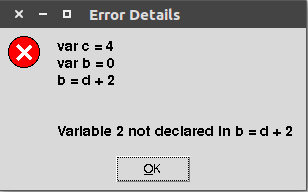
\includegraphics[width=.7\linewidth]{err_dec.png}
      \caption{\label{fig:err_dc}Compilation Error}
   \end{minipage}
\end{figure}


\subsection{Understanding Assembly language }
Let's try to understand a assembly language with a simple Example.This will give us an insight to the underlying algorithms and data structures which is explained later in this \hyperlink{link_algo}{\textbf{section.}}\\\\
\textbf{Assembly language program (8085 microprocessor) to add two 8 bit numbers.}\\
Problem - Write an assembly language program to add two 8 bit numbers stored at address 2050 and address 2051 in 8085 microprocessor. Starting address of program is taken as 2000.\\
\begin{figure}[H]
\centering
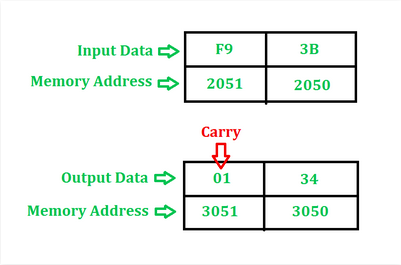
\includegraphics[width=0.5\textwidth]{geeks.png}
\caption{\label{fig:prob}Details related to problem.}
\end{figure}

\textbf{Algorithm}\\
\begin{enumerate}
\item First add contents of memory location 2050 and 2051 using “ADD” instruction and storing at 3050.
\item The carry generated is recovered using “ADC” command and is stored at memory location 3051.
\end{enumerate}
\textbf{Program}\\
        \begin{figure}[H]
\centering
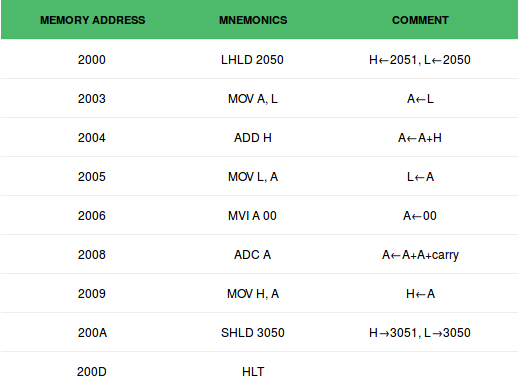
\includegraphics[width=0.4\textwidth]{prog_g.png}
\caption{\label{fig:prob_sol}Assembly Program for the problem.}
\end{figure}
\textbf{Explanation}\\
\begin{enumerate}
\item LHLD 2050 moves the contents of 2050 memory location (3B) in L register and contents of 2051 memory location (F9) in H register.
\item MOV A, L copies contents of L register (3B) to A (Accumulator).
\item ADD H adds contents of A (Accumulator) and H register (F9). The result is stored in A itself. For all arithmetic instructions A is by default an operand and A stores the result as well.
\item MOV L, A copies contents of A (34) to L.
\item MVI A 00 moves immediate data (i.e., 00) to A.
\item ADC A adds contents of A(00), contents of register specified (i.e A) and carry (1). As ADC is also an arithmetic operation, A is by default an operand and A stores the result as well.
\item MOV H, A copies contents of A (01) to H.
\item SHLD 3050 moves the contents of L register (34) in 3050 memory location and contents of H register (01) in 3051 memory location.
\item HLT stops executing the program and halts any further execution.\\\\
\end{enumerate}

Consider another problem which might further clear the understanding of assembly language programming.\\
\textbf{Add the contents of memory locations 200h and 2001h and place the
result in the memory locations 2002h 2003h.}\\\\
LXI H,2000H     ;HL Points 2000H\\
MOV A,M         ;Get the first operand\\
INX H           ;HL points to 2001H\\
ADD M           ;Add second operand\\
INX H           ;HL points to 2002H\\
MOV M,A         ;Store lower byte of result at 2002H\\
MVI A,00        ;Initialize higher byte result with 00H\\
ADC A           ;Add carry in the higher byte\\
INX H           ;HL points 2003h\\
MOV M,A         ;Store the higher nbyte of result at 2003H\\
HLT             ;Terminate the program\\
        




\subsection{Assembler}
An assembly (or assembler) language,often abbreviated asm, is a low-level programming language for a computer, or other programmable device, in which there is a very strong (but often not one-to-one) correspondence between the language and the architecture's machine code instructions. Each assembly language is specific to a particular computer architecture. In contrast, most high-level programming languages are generally portable across multiple architectures but require interpreting or compiling. Assembly language may also be called symbolic machine code.
\begin{figure}[!htb]
\centering
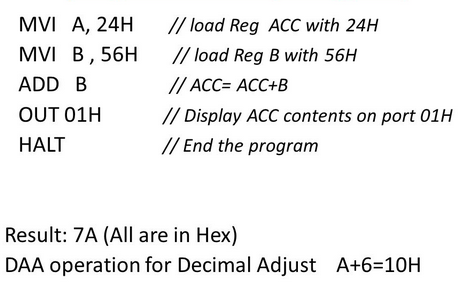
\includegraphics[width=0.5\textwidth]{asmu.png}
\caption{\label{fig:simple_asm} A simple assembly language program(8085).}
\end{figure}


An Assembler converts an assembly language code to an object file or machine language format. An assembler creates object code by translating assembly instruction mnemonics into op-codes, and by resolving symbolic names for memory locations and other entities. Along with this it also includes features of converting macros.
\\An assembler is a translator that translates an assembler program into a conventional machine language program. Basically, the assembler goes through the program one line at a time, and generates machine code for that instruction. Then the assembler proceeds to the next instruction. In this way, the entire machine code program is created.
\\

An assembler primarily serves as the bridge between symbolically coded instructions written in assembly language and the computer processor, memory and other computational components. An assembler works by assembling and converting the source code of assembly language into object code or an object file that constitutes a stream of zeros and ones of machine code, which are directly executable by the processor.
\\Computers ultimately deal in machine language, i.e., binary, to execute programs (assuming that it's not a quantum computer).  This binary is arranged into bit patterns that represent the operation codes that comprise the instruction set for the processor architecture.  However, humans are notoriously bad at working with strings of 1s and 0s for extended periods of time.  So, these operation codes or opcodes are represented symbolically as a set of mnemonics that stand for the opcode.  Opcodes might be operators (commands)  like CMP (compare), ADD (add), MULT (multiply), MOVL (move long (32-bits)), etc. and are typically followed by operands.\\
Assemblers are classified based on the number of times it takes them to read the source code before translating it; there are both single-pass and multi-pass assemblers. Moreover, some high-end assemblers provide enhanced functionality by enabling the use of control statements, data abstraction services and providing support for object-oriented programming structures.
\\
 A computer will not understand any program written in a language, other than its machine language. The programs written in other languages must be translated into the machine language. Such translation is performed with the help of software. A program which translates an assembly language program into a machine language program is called an assembler. If an assembler which runs on a computer and produces the machine codes for the same computer then it is called self assembler or resident assembler. If an assembler that runs on a computer and produces the machine codes for other computer then it is called Cross Assembler.
 \\Below is the picture showing the details of instruction set of 8085 assembler directives.
 \begin{figure}[H]
\centering
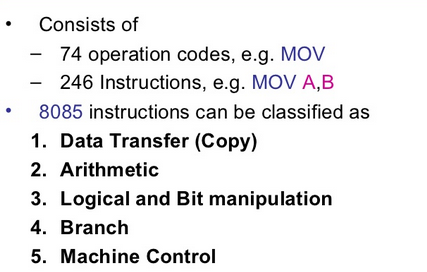
\includegraphics[width=0.5\textwidth]{inst.png}
\caption{\label{fig:inst_set}Synopsis of Instruction set of 8085 .}
\end{figure}
 
Assemblers are further divided into two types: One Pass Assembler and Two Pass Assembler. One pass assembler is the assembler which assigns the memory addresses to the variables and translates the source code into machine code in the first pass simultaneously. A Two Pass Assembler is the assembler which reads the source code twice. In the first pass, it reads all the variables and assigns them memory addresses. In the second pass, it reads the source code and translates the code into object code.\\

There are two types of assemblers based on how many passes through the source are needed to produce the executable program:
\begin{itemize}
  \item  One Pass Assembler: It goes through the code once.
   \item Two Pass Assembler: It goes through the code twice. A table is created with all symbols and their values in the first pass, then the table is used in the second pass to generate code.
\end{itemize}
A two pass assembler has been implemented in this program in python.
Overall working a 2-pass assembler is depicted in the picture given below.


\textbf{Assembler Directives}
\begin{itemize}
\item Assembler directives are pseudo instructions \begin{itemize}
  \item They will not be translated into machine instructions.
  \item They only provide instruction/direction/information to the assembler.
\end{itemize}
\item Basic assembler directives : \begin{itemize}
  \item START : Specify name and starting address for the program
  \item END : Indicate the end of the source program.  \item EQU : The EQU directive is used to replace a number by a symbol. For example: MAXIMUM EQU 99. After using this directive, every appearance of the label “MAXIMUM” in the program will be interpreted by the assembler as the number 99 (MAXIMUM = 99). Symbols may be defined this way only once in the program. The EQU directive is mostly used at the beginning of the program.
\end{itemize}\textbf{Main Data Structures}\begin{itemize}
  \item Operation Code Table (OPTAB)
  \item Location Counter (LOCCTR) \item Symbol Table (SYMTAB) \item Literal Table(LITTAB) 
\end{itemize}\end{itemize}
\textbf{Types of instructions}
\begin{itemize}
  \item Imperative statements
-
indicates an action to be performed during the execution of 
the  assembled  program.  Each  imperative  statement  typically  translates  into  one machine instruction.
  \item Declaration statements
-
the syntax of declaration statements is :\\
\verb|[Label]  DS   <constant>|\\
\verb|[Label]  DC  <value>|\\
The  DS  (short)  for  declare  storage)statement  reserves  areas  of  memory  and 
associates names with them.e.g. 
A    DS   1\\
The  above  statement  reserves  a  memory  area  of  1  word  and  associates  the 
name A with it.\\
The   DC   (short   for   declare   constant)   statement   declare   memory   words 
containing constants.
  \item Assembler Directives- (as explained before).They are Pseudo Instructions.They provide instructions to the assembler itself.
\end{itemize}


\textbf{Instruction Formats}\\
An instruction is a command to the microprocessor to perform a given task on a specified data. Each instruction has two parts: one is task to be performed, called the operation code (opcode), and the second is the data to be operated on, called the operand. The operand (or data) can be specified in various ways. It may include 8-bit (or 16-bit) data, an internal register, a memory location, or 8-bit (or 16-bit) address. In some instructions, the operand is implicit.\\
\begin{itemize}
  \item Addressing modes · Direct addressing (address of operand is given in instruction itself) · Register addressing (one of the operand is general purpose register) · Register indirect addressing (address of operand is specified by register pair) · Immediate addressing (operand - data is specified in the instruction itself) · Implicit addressing (mostly the operation operates on the contents of accumulator)
  \item Program relocation · It is desirable to load and run several programs and resources at the same time · The system must be able to load programs into memory wherever there is room · The exact starting address of the program is not known until load time. · The assembler can identify (for the loader) those parts of the program that need modification. · An object program that contains this type of modification information necessary to perform modification is called a re-locatable program.
\end{itemize}
\begin{figure}[!htb]
\centering
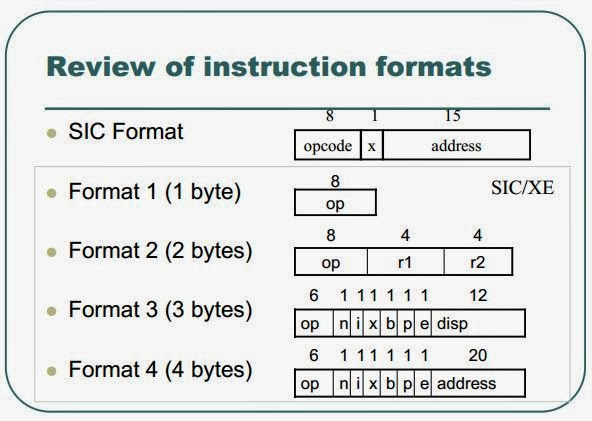
\includegraphics[width=0.8\textwidth]{instruction.jpeg}
\caption{\label{fig:instruction_format}Instruction formats.}
\end{figure}

\textbf{Literals}\\
It is convenient for the programmer to be able to write the value of a constant operand as a part of the instruction that uses it. Such an operand is called a literal. In this assembler language notation, a literal is identified with the prefix ‘=’, which is followed by a specification of the literal value.\\
\textbf{The difference between literal operands and immediate operands}\\
\begin{itemize}
  \item For literal operand we use ‘=’ as prefix, and with immediate operand we use \verb|‘#’| as prefix
  \item During immediate addressing, the operand value is assembled as part of the machine instruction, and there is no memory reference.\item With a literal, the assembler generates the specified value as a constant at some other memory location.
\end{itemize}
\subsubsection{Design Specification of an assembler}
We use a four steps approach to develop a design specification for an assembler.
\begin{itemize}
\item Identify The information necessary to perform a task.\item Design a suitable data structure to record the information.\item Determine the processing necessary to obtain and maintain the information. \item Determine the processing necessary to perform the task . 
\end{itemize}

\begin{figure}[H]
\centering
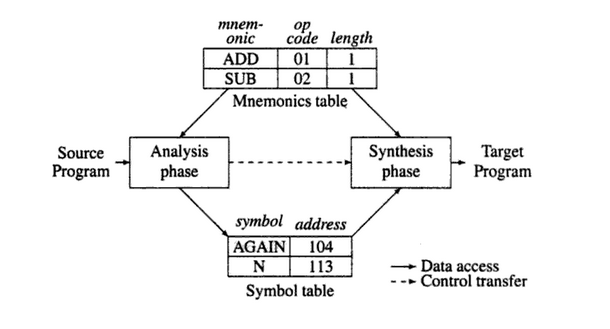
\includegraphics[width=0.8\textwidth]{datas.png}
\caption{\label{fig:data_s}Data structures of the assembler.}
\end{figure}



\subsubsection{Overall Steps Taken}
%STEPS TAKEN
\begin{itemize}
    \item  Convert mnemonic operation codes to their machine language equivalents
  \item   Convert symbolic operands to their equivalent machine addresses
    \item Build the machine instructions in the proper format
    \item Convert the data constants to internal machine representations
    \item Write the object program and the assembly listing\end{itemize}
\hypertarget{link_algo}{\subsubsection{ Explanation of the whole process}}
\begin{enumerate}
\item \textbf{Identify the information necessary to perform a task.}\\The fundamental information requirements arise in the synthesis phase of an
assembler. Hence it is best to begin by considering the information requirements of
the synthesis tasks. The information is collected during analysis or derived during
synthesis phase. For e.g. Consider the assembly statement  :\\MOVER BREG , ONE\\Following information is required to synthesize the machine instruction
corresponding to this statement:\begin{itemize}
  \item Address of the memory word with which name ONE is associated.
  \item Machine operation code corresponding to the mnemonic MOVER.
\end{itemize}The first item of information depends on the source program. Hence it is made
available by analysis phase. The second item of information does not depend on the
source program , it merely depends on the assembly language. Hence the synthesis
phase can determine this information for itself.
\item \textbf{Design a suitable data structure to record the information.}\\ The data structures SYMTAB(for symbol table),OPTAB(for operation code table/ mnemonics table),LOCCTR(for location counter) are to be used.\\\\\textbf{SYMTAB}
 \begin{itemize}\item Fields : symbol name, address.
 \item It is a dynamic table built by analysis phase.
 \item To indicate error conditions (Ex: multiple define).
 \item Insert, delete and search allowed.
 \item Usually use a hash table.  \end{itemize}\textbf{OPTABLE}
 \begin{itemize}\item Fields: Mnemonic, opcode, length.
 \item It is a static table.
 \item Array or hash table.
 \item Usually use a hash table (mnemonic opcode as key).
   \end{itemize}\textbf{LOCCTR}
 \begin{itemize}\item Initialize to be the beginning address specified in the “START” statement.
 \item LOCCTR =LOCCTR + (instruction length).
 \item The current value of LOCCTR gives the address to the label/symbol encountered.
   \end{itemize} Below are the instances of the these data structures according to the algorithm after pass1 for the program:\\\\var a = 0\\
loop 3\\
a = a + 1\\
endloop\\\\ Assembly code produced is:\\MVI D, ='0'\\
MOV \#a,D\\
PUSH E\\
MVI E, 3\\
LDA \#a\\
ADI 1\\
STA \#a\\
MOV A,E\\
SUI 1\\
MOV E,A\\
JNZ ~~~loop0\\
POP E\\
END\\
a DS 1\\
='0'\\ And the instances of symbol Table and LIteral table is:\\\begin{figure}[H]
\centering
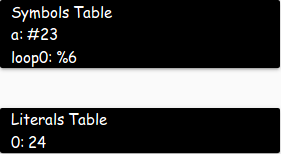
\includegraphics[width=0.5\textwidth]{sym_table.png}
\caption{\label{fig:tables_dict}Data structures after pass1 for above program.}
\end{figure}
\item \textbf{Determine the processing necessary to obtain and maintain the information.}\\For building symbol table during analysis phase, it is necessary to determine the
addresses with which the symbol names used in a program is associated. It is
possible to determine some addresses directly e.g. the address of the first instruction
in the program, however others must be inferred. To determine the address of an
instruction, it is required to fix the addresses of all instructions preceding it. This
function is called memory allocation.\\\\To implement memory allocation , the data structure location counter is used. The
location counter is always made to contain the address of the next memory word in
the target program..It is initialized to the constant specified in the START statement.
Whenever the analysis phase sees a label in an assembly statement, it enters the
label and the contents of LC in a new entry of the symbol table. It then finds the
number of memory words required by the assembly statement and updates the LC
contents. The information about the length of different instructions is included in the
opcode/ mnemonics table.\\The processing involved in maintaining the location counter is referred as LC processing.
\item \textbf{Determine the processing necessary to perform the task.}\\The tasks performed by the analysis and synthesis phases are as follows:\\\\\textbf{Analysis Phase}\begin{enumerate}
\item Isolate the label, mnemonic opcode and operand fields of a statement.
\item If a label is present, enter the pair 9 symbol, <LC contents>) in a new entry of
Symbol table.
\item Check validity of the mnemonic opcode through a look-up in the Opcode table.
\item Perform LC processing i.e. update the value contained in LC by considering the
opcode and operands of the statements.
\end{enumerate}\textbf{Synthesis Phase}\begin{enumerate}
\item Obtain the machine opcode corresponding to the mnemonic from the Opcode table.
\item Obtain address of a memory operand from the symbol table.
\item Check validity of the mnemonic opcode through a look-up in the Opcode table.
\item Perform LC processing i.e. update the value contained in LC by considering the
opcode and operands of the statements.
\end{enumerate}
\end{enumerate}

\subsubsection{One Pass Assemblers}
A one pass assembler passes over the source file exactly once, in the same pass collecting the labels, resolving future references and doing the actual assembly. The difficult part is to resolve future label references (the problem of forward referencing) and assemble code in one pass.Below is the diagrammatic representation of steps covered in one-pass assemblers.To understand one pass assemblers, we must first understand 2-pass assemblers for more insight as it is just a variation of two pass assemblers in pursuit of optimizing the process complexity.\\LC processing and construction of the symbol table proceeds with analysis phase.
The problem of forward references is tackled using a process called backpatching. The
operand field of an instruction containing a forward reference is left blank initially.The address of the forward referenced symbol is put into this field when its definition is
encountered. The instruction corresponding to the statement\\MOVER BREG , ONE \\can be only partially synthesize since ONE is a forward reference. Hence the instruction
opcode and address of BREG will be assembled to reside in location 101. The need for
inserting the second operand’s address at a later stage can be indicated by adding an entry
to the Table of Incomplete Instructions (TII).This entry is a pair ( <instruction
address>, <symbol>), e.g. (101. ONE) in this case.\\By the time END statement is processed, the symbol table would contain the addresses of
all symbols defined in the source program and TII would contain information describing
all forward references. The assembler can now process each entry in TII to complete the
concerned instruction.
\begin{figure}[!htb]
\centering
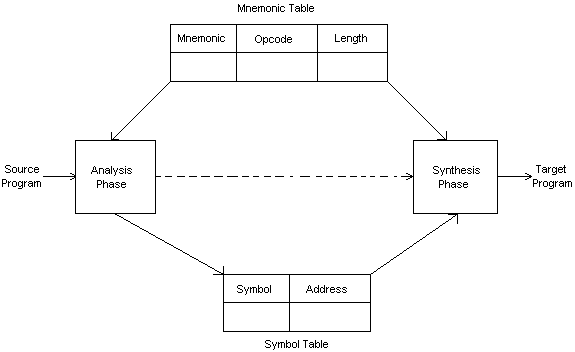
\includegraphics[width=0.8\textwidth]{one_pass.png}
\caption{\label{fig:one_pass}One pass Assemblers.}
\end{figure}

\*
\textbf{Forward reference in one pass assembler}\\
\begin{itemize}
  \item Omits the operand address if the symbol has not yet been defined
  \item Enters this undefined symbol into SYMTAB and indicates that it is undefined \item Adds the address of this operand address to a list of forward references associated with the SYMTAB entry \item When the definition for the symbol is encountered, scans the reference list and inserts the address. \item At the end of the program, reports the error if there are still SYMTAB entries indicated undefined symbols.
\end{itemize}

\subsubsection{Two Pass Assemblers}
% 2-PASS ASSEMBLERS 
wo   pass   translation   of   an   assembly   language   program   can   handle   forward 
references easily. LC processing is performed in the first pass and symbols defined in the 
program  are  entered  into  the  symbol  table.  The  second  pass  synthesizes  the  target  form 
using the address information found in the symbol table. In effect, the first pass performs 
the 
analysis  of  the  source  program  while  the  second  pass  performs  synthesis  of  target 
program.  The  first  pass  constructs  an  intermediate  representation  (IR)  of  the  source 
program for use by the second pass. \\
 Consider an assembler instruction like the following:-\\

          JMP  LATER\\
                 ...\\
                   ...\\
LATER:\\

This is known as a forward reference. If the assembler is processing the file one line at a time, then it doesn't know where LATER is when it first encounters the jump instruction. So, it doesn't know if the jump is a short jump, a near jump or a far jump. There is a large difference amongst these instructions. They are 2, 3, and 5 bytes long respectively. The assembler would have to guess how far away the instruction is in order to generate the correct instruction. If the assembler guesses wrong, then the addresses for all other labels later in the program woulds be wrong, and the code would have to be regenerated. Or, the assembler could alway choose the worst case. But this would mean generating inefficiency in the program, since all jumps would be considered far jumps and would be 5 bytes long, where actually most jumps are short jumps, which are only 2 bytes long.

So, what is to be done to allow the assembler to generate the correct instruction? Answer: scan the code twice. The first time, just count how long the machine code instructions will be, just to find out the addresses of all the labels. Also, create a table that has a list of all the addresses and where they will be in the program. This table is known as the symbol table. On the second scan, generate the machine code, and use the symbol table to determine how far away jump labels are, and to generate the most efficient instruction.

This is known as a two-pass assembler. Each pass scans the program, the first pass generates the symbol table and the second pass generates the machine code. 
\begin{figure}[H]
\centering
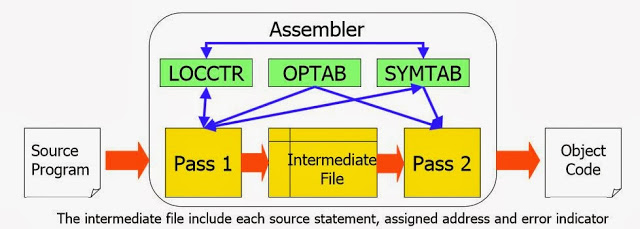
\includegraphics[width=0.8\textwidth]{assembler.jpeg}
\caption{\label{fig:2_pass}working of a 2-pass assembler.}
\end{figure}

The two pass assembler performs two passes over the source program.\\

In the first pass, it reads the entire source program, looking only for label definitions. All the labels are collected, assigned address, and placed in the symbol table in this pass, no instructions as assembled and at the end the symbol table should contain all the labels defined in the program. To assign address to labels, the assembles maintains a Location Counter (LC).\\

In the second pass the instructions are again read and are assembled using the symbol table. Basically, the assembler goes through the program one line at a time, and generates machine code for that instruction. Then the assembler proceeds to the next instruction. In this way, the entire machine code program is created. For most instructions this process works fine, for example for instructions that only reference registers, the assembler can compute the machine code easily, since the assembler knows where the registers are.\\
Picture below shows the tasks performed on a broader basis.

\begin{figure}[H]
\centering
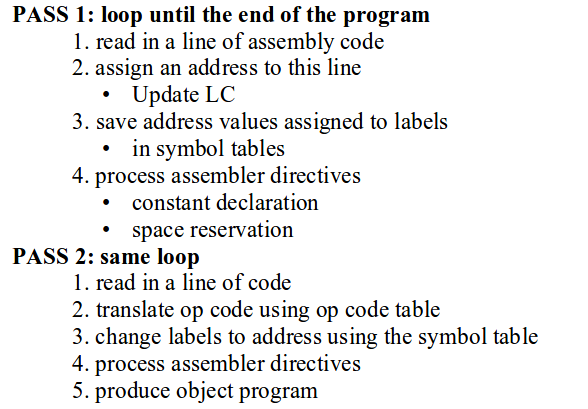
\includegraphics[width=0.6\textwidth]{tasks2.png}
\caption{\label{fig:task_2pass} Tasks performed in 2-Pass assembler.}
\end{figure}
\subsubsection{Difference between One Pass and Two Pass Assemblers}
The difference between one pass and two pass assemblers are:-\\A one pass assembler passes over the source file exactly once, in the same pass collecting the labels, resolving future references and doing the actual assembly. The difficult part is to resolve future label references (the problem of forward referencing) and assemble code in one pass. The one pass assembler prepares an intermediate file, which is used as input by the two pass assembler.\\A two pass assembler does two passes over the source file (the second pass can be over an intermediate file generated in the first pass of the assembler). In the first pass all it does is looks for label definitions and introduces them in the symbol table (a dynamic table which includes the label name and address for each label in the source program). In the second pass, after the symbol table is complete, it does the actual assembly by translating the operations into machine codes and so on.
\subsection{Linker}
In high level languages, some built in header files or libraries are stored. These libraries are predefined and these contain basic functions which are essential for executing the program. These functions are linked to the libraries by a program called Linker. If linker does not find a library of a function then it informs to compiler and then compiler generates an error. The compiler automatically invokes the linker as the last step in compiling a program.\\Computer programs typically are composed of several parts or modules; these parts/modules need not all be contained within a single object file, and in such cases refer to each other by means of symbols. Typically, an object file can contain three kinds of symbols:
\begin{itemize}
  \item defined "external" symbols, sometimes called "public" or "entry" symbols, which allow it to be called by other modules, 
  \item undefined "external" symbols, which reference other modules where these symbols are defined, and \item local symbols, used internally within the object file to facilitate relocation.
\end{itemize}
For most compilers, each object file is the result of compiling one input source code file. When a program comprises multiple object files, the linker combines these files into a unified executable program, resolving the symbols as it goes along.\\Linkers can take objects from a collection called a library. Some linkers do not include the whole library in the output; they include only its symbols that are referenced from other object files or libraries. Libraries exist for diverse purposes, and one or more system libraries are usually linked in by default.\\The linker also takes care of arranging the objects in a program's address space. This may involve relocating code that assumes a specific base address to another base. Since a compiler seldom knows where an object will reside, it often assumes a fixed base location (for example, zero). Relocating machine code may involve re-targeting of absolute jumps, loads and stores.\\The executable output by the linker may need another relocation pass when it is finally loaded into memory (just before execution). This pass is usually omitted on hardware offering virtual memory: every program is put into its own address space, so there is no conflict even if all programs load at the same base address. This pass may also be omitted if the executable is a position independent executable.\\ 
Not built in libraries, it also links the user defined functions to the user defined libraries. Usually a longer program is divided into smaller subprograms called modules. And these modules must be combined to execute the program. The process of combining the modules is done by the linker.\\

\subsubsection{Tasks of a Linker:-}
\begin{itemize}
  \item Searches the program to find library routines used by 
program, e.g. 
printf
(), math routines,...
  \item etermines the memory locations that code from each 
module will occupy and relocates its instructions by 
adjusting absolute references.\item Resolves references among files
\end{itemize}

\begin{figure}[H]
\centering
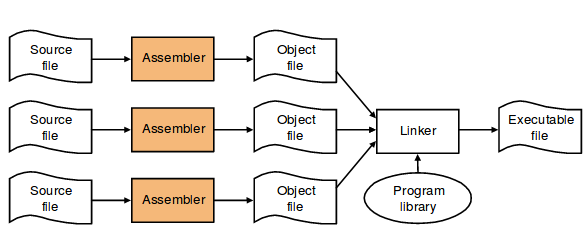
\includegraphics[width=0.8\textwidth]{linker.png}
\caption{\label{fig:linker} Process for producing an executable file using linker}
\end{figure}
\subsubsection{Linking Requirements}
\begin{itemize}
  \item All program units are translated separately.
  \item Hence, all 
sub program calls  and common variable 
reference require linking. \item Programs are 
nested
in main program. \item Procedure reference do not require linking
, they can be 
handled using 
relocation.\item Build in functions require linking. \item Linker processes all object modules being linked and builds a 
table of all public definition and load time address. \item Name Table (NTAB)  \begin{itemize}
  \item  
Symbol
: Symbol Name for external reference or object 
module.
  \item 
Linked Address
: For public definition contains 
link-address
. 
For object  module  contains 
link-origin
.
\end{itemize}  \item Most information in NTAB is derived from LINKTAB entries 
with type=PD.
\end{itemize}

\subsubsection{Algorithm Of a LInker}
\begin{enumerate}
\item program-linked-origin:= <link origin> from linker command.
\item For each object module \begin{itemize}
  \item t-origin:= translated origin of object module. OM-size:=size of the object module;
  \item Relocation-factor:= program-linked-origin–t-origin. \item Read the machine language program in 
work-area
. \item Read LINKTAB of the object module. \item For each LINKTAB entry with type = PD\\name:= symbol;\\linked-address
:= 
translated-address
+ 
relocation-factor
;\\enter(
name,linked-address
) in NTAB.\item Enter (object module name, 
program-linked-origin
) in NTAB; \item  
program-linked-origin
:= 
program-linked-origin
+ 
OM-size
;

\end{itemize}
\item for each object module \begin{itemize}
  \item  
t-origin
:= translated origin of the object 
module.
  \item For each LINKTAB entry with type=EXT \begin{itemize}
  \item address-in-work-area
:= 
address of 
work-area
+ 
program-linked-origin
–
<
link-origin
> + translated address 
–
`
t-origin
;
  \item Search symbol in NTAB and copy its
linked address. Add the linked address 
to the operand address in the word with 
the address 
address-in-work-area
.
\end{itemize}
\end{itemize}
\end{enumerate}
\textbf{Example}\\
\begin{figure}[H]
\centering
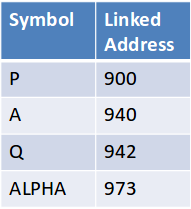
\includegraphics[width=0.3\textwidth]{ntab.png}
\caption{\label{fig:ex_link} NTAB information.}
\end{figure}
\begin{itemize}
  \item While linking program P and 
program Q with 
linked-origin
=900, NTAB 
contains above information:   
  \item Work-area
= 300. \item When LINKTAB of alpha is 
processed during linking, 
address-in-work-area
:= 300 + 
900 
-
900 + 518 
–
500. 
i.e
318. \item Hence linked address of ALPHA 
is 973, is copied from NTAB 
entry of ALPHA and added to 
word in address 318.
\end{itemize}
\subsubsection{Relocation}
As the compiler has no information on the layout of objects in the final output, it cannot take advantage of shorter or more efficient instructions that place a requirement on the address of another object. For example, a jump instruction can reference an absolute address or an offset from the current location, and the offset could be expressed with different lengths depending on the distance to the target. By generating the most conservative instruction (usually the largest relative or absolute variant, depending on platform) and adding relaxation hints, it is possible to substitute shorter or more efficient instructions during the final link. This step can be performed only after all input objects have been read and assigned temporary addresses; the linker relaxation pass subsequently reassigns addresses, which may in turn allow more relaxations to occur. In general, the substituted sequences are shorter, which allows this process to always converge on the best solution given a fixed order of objects; if this is not the case, relaxations can conflict, and the linker needs to weigh the advantages of either option.\\While instruction relaxation typically occurs at link-time, inner-module relaxation can already take place as part of the optimising process at compile-time. In some cases, relaxation can also occur at load-time as part of the relocation process or combined with dynamic dead-code elimination techniques.\\\\
Consider a program consisting of 2 different files and one of them having extern variable to use variable of another file.\\
First file contains:\\
\\global a = 5\\\\
while 2nd file contains \\\\
extern a\\
a = a + 2\\\\
Output given by linker:\\
\begin{figure}[H]
\centering
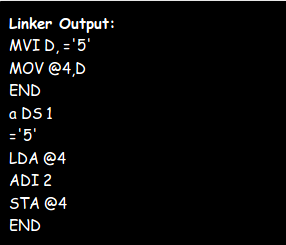
\includegraphics[width=0.5\textwidth]{link_out.png}
\caption{\label{fig:link_out} LInker output for the given program.}
\end{figure}


\subsection{Loader}
Loader is a program that loads machine codes of a program into the system memory. In Computing, a loader is the part of an Operating System that is responsible for loading programs. It is one of the essential stages in the process of starting a program. Because it places programs into memory and prepares them for execution. Loading a program involves reading the contents of executable file into memory.  Once loading is complete, the operating system starts the program by passing control to the loaded program code. All operating systems that support program loading have loaders. In many operating systems the loader is permanently resident in memory. \\In computer systems a loader is the part of an operating system that is responsible for loading programs and libraries. It is one of the essential stages in the process of starting a program, as it places programs into memory and prepares them for execution. Loading a program involves reading the contents of the executable file containing the program instructions into memory, and then carrying out other required preparatory tasks to prepare the executable for running. Once loading is complete, the operating system starts the program by passing control to the loaded program code.\\All operating systems that support program loading have loaders, apart from highly specialized computer systems that only have a fixed set of specialized programs. Embedded systems typically do not have loaders, and instead the code executes directly from ROM. In order to load the operating system itself, as part of booting, a specialized boot loader is used. In many operating systems the loader is permanently resident in memory, although some operating systems that support virtual memory may allow the loader to be located in a region of memory that is pageable.\\In the case of operating systems that support virtual memory, the loader may not actually copy the contents of executable files into memory, but rather may simply declare to the virtual memory subsystem that there is a mapping between a region of memory allocated to contain the running program's code and the contents of the associated executable file. (See memory-mapped file.) The virtual memory subsystem is then made aware that pages with that region of memory need to be filled on demand if and when program execution actually hits those areas of unfilled memory. This may mean parts of a program's code are not actually copied into memory until they are actually used, and unused code may never be loaded into memory at all.\\It is the part of the OS that brings an executable file 
residing on disk into memory and starts it running.\\
The main task of the loader is to bring binary executable image into main
memory and bind the relocatable addresses into absolute addresses.\\\\
The binary image of a program consists of following parts :-
\begin{itemize}
  \item Header – It shows the type of file (executable or library file).
  \item Text – It shows the actual code of the program \item List of shared libraries - libraries that have been used in the object
file.
\end{itemize}
\subsubsection{Steps of carrying out Loading:-}
\begin{itemize}
  \item Read executable file’s header to determine the size of 
text and data segments.
  \item Create a new address space for the program.\item Copies instructions and data into address space. \item Copies arguments passed to the program on the stack.\item Initializes the machine registers including the stack ptr. \item Jumps to a startup routine that copies the program’s 
arguments from the stack to registers and calls the 
program’s main routine
\end{itemize}
\begin{figure}[H]
\centering
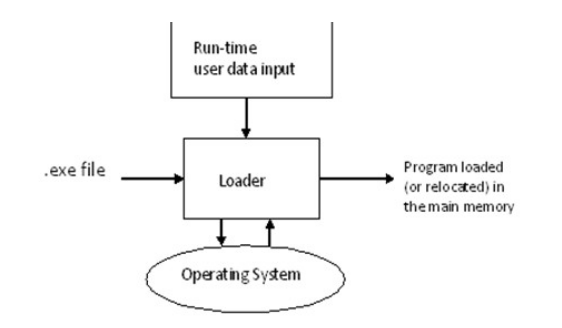
\includegraphics[width=0.8\textwidth]{loader.png}
\caption{\label{fig:loader} Functioning of a Loader.}
\end{figure}

\subsubsection{Design of an Absolute Loader}

An absolute object file consists of three part-
\begin{enumerate}
\item The start address of the program
\item The object instructions
\item The address of the first executable instruction. This is placed in the
object file by assembler in response to the END directive. It is either the
address specified by the END or, in the absence of such an address is
identical to the first address of the program.
\end{enumerate}
The loader reads the first item and loads the rest of object file into
successive memory locations.

% \subsection{How to add Lists}

% You can make lists with automatic numbering \dots

% \begin{enumerate}
% \item Like this,
% \item and like this.
% \end{enumerate}
% \dots or bullet points \dots
% \begin{itemize}
% \item Like this,
% \item and like this.
% \end{itemize}

% \subsection{How to add Citations and a References List}

% You can upload a \verb|.bib| file containing your BibTeX entries, created with JabRef; or import your \href{https://www.overleaf.com/blog/184}{Mendeley}, CiteULike or Zotero library as a \verb|.bib| file. You can then cite entries from it, like this: \cite{greenwade93}. Just remember to specify a bibliography style, as well as the filename of the \verb|.bib|.

% You can find a \href{https://www.overleaf.com/help/97-how-to-include-a-bibliography-using-bibtex}{video tutorial here} to learn more about BibTeX.

% We hope you find Overleaf useful, and please let us know if you have any feedback using the help menu above --- or use the contact form at \url{https://www.overleaf.com/contact}!

% \bibliographystyle{alpha}

% \bibliography{sample}
\section{Bibliography}
\begin{itemize}
\item Systems Programming and Operating Systems
by Dhananjay Dhamdhere (\url{https://books.google.co.in/books?cad=0&id=s7zgF7InxIgC&printsec=frontcover&source=gbs_ge_summary_r#v=onepage&q&f=true})
\item \href{https://www.slideshare.net/ShubhamShah001/two-pass-assembler}{2-pass Assembler explanation }
\item wiki-assembler(\url{https://en.wikipedia.org/wiki/Assembly_language#Assembler})
\item Linker and Loader by John R. Levine (\url{http://www.becbapatla.ac.in/cse/naveenv/docs/LL1.pdf})
\end{itemize}

\end{document}